
\begin{table}[t]
  
  
\begin{tabularx}{\columnwidth}{Xcccccc}
& \multicolumn{6}{c}{\normalsize{\textbf{Attribute Count}}} \\
& {\normalsize{\textbf{0}}} 
& {\normalsize{\textbf{1}}} 
& {\normalsize{\textbf{2}}} 
& {\normalsize{\textbf{3}}} 
& {\normalsize{\textbf{4}}} 
& {\normalsize{\textbf{5}}} \\ \midrule
Unreasonable Fear & 48&33&16&2&0&0 \\
Uncomfortable & 24&19&18&16&12&11 \\
Interested in changing & 18&22&19&21&11&10 \\

\end{tabularx}

  
  \caption{\textbf{Summary of survey results.} Aggregates are shown for the
    three specific questions addressed in Section~\ref{subsec-surveyresults}.
    All values are percentages.}
  
  \label{table-surveysummary}

\end{table}

\section{Evaluation}
\label{sec-evaluation}

Our evaluation of \PocketMocker{} has three aims. First, we establish that
\PocketMocker{} is desirable through a survey of 91 smartphone users
(\S\ref{subsec-survey}). Second, we show that \PocketMocker{} works, by
mocking several popular Android apps, and briefly discuss the overhead of the
mocking process (\S\ref{subsec-mockingapps}). Finally, we demonstrate that
\PocketMocker{} is usable through a small user experiment where several
volunteers were able to use \PocketMocker{} to mock a pedometer app
(\S\ref{subsec-usability}).

\subsection{Users Want to Use \PocketMocker{}}
\label{subsec-survey}

Before beginning \PocketMocker{} development, to gauge interest in mocking we
distributed an IRB-approved survey to students, faculty and staff at our
university. No incentives were provided for completing the survey, and all
respondents were required to indicate consent before proceeding to the
questions. Over four days, we recorded 91 responses.

\subsubsection{Survey Questions}

Table~\ref{table-surveyquestions} summarizes the survey we distributed. It
had three parts, each consisting of questions concerning five personal
attributes: home location, weight, activity level, income level, and
sociability. The goal of the first part was to assess how aware respondents
were of the information smartphones apps could collect about them.
Respondents were instructed to assume that the hypothetical app had been
installed and granted the permissions it requested. The goal of the second
part of the survey was to assess how comfortable respondents were with the
data smartphone apps could collect about them. Finally, the third part
assessed interest in mocking by determining how interested respondents were
in misleading apps about the five attributes.

We intentionally chose a range of attributes. We considered home address and
social network as straightforward to determine for an app with the right
permissions, in this case the ability to track user's location (home address)
or observe who they communicate with (social network). At the time we
considered activity level to be more difficult to determine, although now
that activity recognition has been integrated into widely-available libraries
such as Google Play Services this may be much simpler to measure using the
accelerometer. Finally, we chose two attributes that we were not sure could
actually be determined by smartphones: income and weight.

Based on the capabilities of current smartphones we classified answers to the
accuracy questions as either reasonable or unreasonable. As an example, we
considered it unreasonable that an app could know a user's income to within
\$1 / year or their weight to within 1 lb. However, it is possible that by
using the accelerometer and studying a user's gait their weight could be
estimated, and the widespread adoption of smartphone-based payment systems
such as Google Wallet along with socioeconomic map-matching may make income
levels estimable soon. So even the answers we marked as unreasonable may not
remain so for long.

\subsubsection{Survey Results}
\label{subsec-surveyresults}

Table~\ref{table-surveyresults} shows detailed results of our mocking survey.
When analyzing the results, we were interested in three questions matching
the three sections of our survey. First, how reasonable were respondents
fears about information that apps might be able to determine? Second, how
comfortable were they sharing data with apps? And finally, were respondents
interested in modifying the data-driven impressions app might form of them?
Table~\ref{table-surveysummary} reports aggregate results relevant to these
three questions.

First, we found that respondents to be reasonably suspicious of what apps
might know about them, with 52\% indicating that an app might know at least
one personal attribute to a level that we marked as unreasonable today but
only 18\% indicating that apps might know two attributes of unreasonable
levels. The two unreasonable attributes most-frequently reported as knowable
by respondents were their income to \$100 / year (24\%), and the quantity and
type of the exercise they engaged in (20\%). Overall, users' intuition about
what attributes were easy to determine and what were hard matched ours,
reflected by the accuracy percentages in the table. No users thought an
app would not be able to determine anything about their home address,
whereas 39\% didn't think an app could determine anything about their weight.

Second, our survey showed that many respondents were uncomfortable with
smartphones knowing these aspects of their personal lives. Only 24\% were
comfortable, defined as a score of 2 or above on the 1--5 scale, with all
five attributes, and a majority (57\%) were uncomfortable with two or more.
Our results match the privacy concerns reported by smartphone users to other
surveys~\cite{truste-privacy}. Reported comfort levels on individual
attributes were also interesting, with users seeming the least comfortable
with smartphones knowing their home address---which is possible---and their
income---which, at least today, may not be. Comfort levels regarding
knowledge of a users social network were evenly distributed.

Finally, when asked about mocking, of the 91 users that completed the survey,
82\% wanted to mock at least one attribute and 60\% wanted to mock two, with
mocking users requesting an average of 2.6 mocking attributes each. Interest
in mocking different attributes was well distributed, with the percentage of
mocking responses per attribute varying from a low of 26\% for activity level
to a high of 66\% for income.

Unsurprisingly, users were most interested in mocking attributes that they
were uncomfortable with their smartphone knowing, such as home address and
income level. Surprisingly, most users seemed to want to appear to make
\textit{less} money than they actually do, which is not what we expected. We
speculate that this may be because users believe that they will see fewer ads
if advertisers believe that they are poor. In any case, it shows that it may
be difficult to determine what changes users see as desirable.

\newpage
Overall, however, the results lead us to the conclusion that smartphone
users:
\begin{itemize}

\item have reasonable expectations about what smartphone apps might be able to
learn about them,
\item are uncomfortable with apps knowing these things,
\item and are interested in misleading apps.

\end{itemize}

\subsection{\PocketMocker{} Can Mock Smartphone Apps}
\label{subsec-mockingapps}

Having shown that mocking is desirable, we continue by demonstrating that our
\PocketMocker{} prototype works by using it to mock three smartphone apps. In
each case we describe the app, discuss why users might want to mock it,
describe our specific mocking objective and whether it was achieved.

\subsubsection{Mocking Maps}

\begin{figure*}[t]

\begin{subfigure}[t]{2.33in}
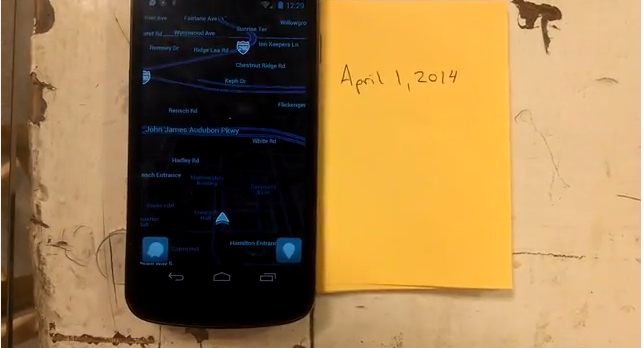
\includegraphics[width=2.33in]{./figures/apps/waze/waze1.png}
\caption{}
\end{subfigure}%
\begin{subfigure}[t]{2.33in}
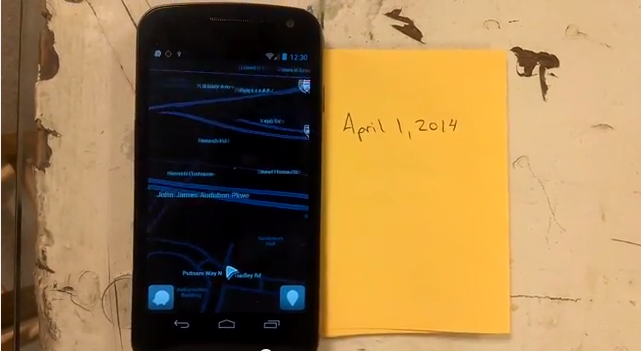
\includegraphics[width=2.33in]{./figures/apps/waze/waze2.png}
\caption{}
\end{subfigure}%
\begin{subfigure}[t]{2.33in}
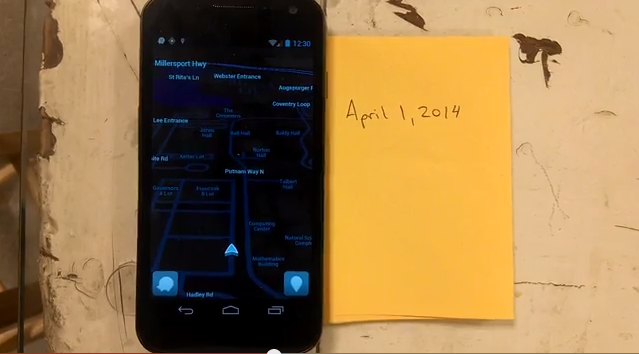
\includegraphics[width=2.33in]{./figures/apps/waze/waze3.png}
\caption{}
\end{subfigure}%

\caption{\textbf{Mocking Waze.} The screenshots demonstrate that we were
successfully able to mock the Waze maps app. As the mocking trace is
replayed, the phone remains stationary on the desk, but Waze thinks that the
user is walking around.}

\label{fig-mocking-waze}

\end{figure*}

\begin{table}
\begin{tabularx}{3.33in}{lX}
\textbf{App} & Waze Social Maps \& Traffic \\ \toprule
\textbf{Installs} & 10--50~million \\
\textbf{Mocking Objective} & Mock location \\ \midrule
\textbf{Trace Length} & 2 minutes 27 seconds \\
\textbf{Trace Size} & 516~K \\
\textbf{Location Mocks} & 117 \\
\textbf{Sensors Used} & {\small GPS, Gyroscope, Accelerometer} \\
\textbf{Sensor Mocks} & 2773 \\
\textbf{Wifi Scan Mocks} & 115 \\
\textbf{Cell Location Mocks} & 117 \\
\textbf{Video URL} &
\hyperlink{http://youtu.be/GIqXP6b769c}{\texttt{http://youtu.be/GIqXP6b769c}} \\

\end{tabularx}

\caption{\textbf{Mocking Waze.} Details of our Waze mocking trace.}

\label{table-mocking-waze}

\end{table}

As a first example of \PocketMocker{} in action, we mock the Waze maps
app~\cite{waze-playstore-url}. Waze describes itself as a community-based
traffic and navigation app allowing ``millions of drivers from across the
globe joining forces to outsmart traffic, save time, gas money, and improve
daily commuting for all''.

Our objective in mocking Waze was to show that \PocketMocker{} can provide
fine-grained location to the many smartphone apps that use location to
customize the user experience. Given the amount of information smartphone
users' location can reveal about them, it is important for \PocketMocker{} to
effectively support location mocking. In our next mocking example we show the
effect that mocked locations can have on an unsuspecting app.

To mock Waze, We first recorded a mocking trace of a walk around campus,
described in more detail in Table~\ref{table-mocking-waze}.  This included
tracking location, connectivity, and sensor data from the gyroscope and
accelerometer that Waze utilizes. We then placed the smartphone on a desk,
initiated a replay session and launched the Waze app.
Figure~\ref{fig-mocking-waze} shows three screenshots of Waze being mocked,
showing that the users location is being updated to follow the trace despite
the smartphone not moving. An anonymized video of our successful Waze mocking
session is also available at
\hyperlink{http://youtu.be/GIqXP6b769c}{\texttt{http://youtu.be/GIqXP6b769c}}.

\subsubsection{Mocking checkins}

As an example of a more realistic mocking scenario, we used \PocketMocker{}
to mock the popular Facebook app~\cite{facebook-playstore-url}. Facebook is
the world's largest social networking site and its Android app is quite
popular, with the Play Store estimating between 500~million and 1~billion
installs. People use Facebook to share content and stay in touch with
friends.

Our objective in mocking Facebook was to initiate a check-in at a mocked
location. Like FourSquare, the Facebook app contains a check-in feature
allowing users to easily report that they are at a particular location, with
check-ins being posted to their news feed and visible to their friends.
Initiating mocked check-ins could be done for several reasons. Some Facebook
users may want to appear more social than they actually are by initiating
mocked check-ins at popular bars or clubs even on nights when they would
prefer to stay home. Others may use mocked check-ins to compete for
promotions provided by locations, or to compete for coveted status such as
the ``Mayorships'' provided by FourSquare. Some FourSquare users have become
so interested in earning the title of Mayor at a particular location that
there is actually an entire website devoted to helping
them\footnote{\hyperlink{http://whenwillibemayor.com/}{\texttt{http://whenwillibemayor.com/}}}.

To mock a Facebook check-in, we recorded a mocking trace of a walk to the
nearby Starbucks, which included location, connectivity, and sensor data from
the accelerometer. Because the trace was collected outdoors, no Wifi scan
data was captured. We then placed the smartphone on a desk, initiated a
replay session and launched the Facebook app.
Figure~\ref{fig-mocking-facebook} shows three screenshows of Facebook being
mocked demonstrating that Facebook did allow us to check in at Starbucks at
the end of the trace despite the smartphone not being located nearby. We did
record a video of the mocking process, but due to the amount of personal
information revealed by Facebook we were not able to anonymize it
sufficiently.

\begin{figure*}[t]

\begin{subfigure}[t]{2.33in}
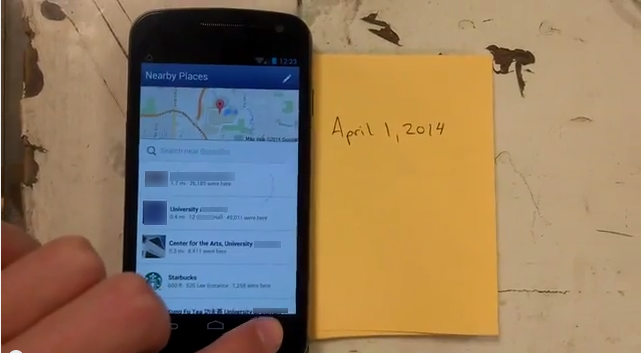
\includegraphics[width=2.33in]{./figures/apps/facebook/facebook1.png}
\caption{}
\end{subfigure}%
\begin{subfigure}[t]{2.33in}
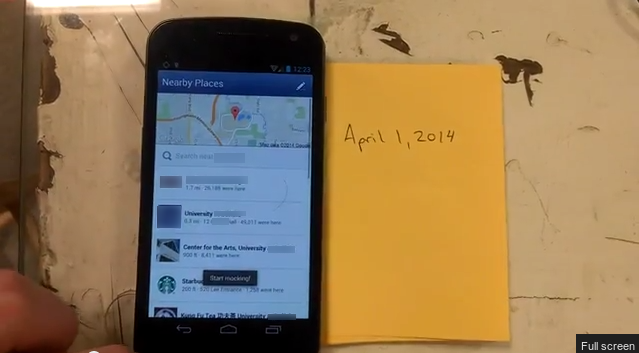
\includegraphics[width=2.33in]{./figures/apps/facebook/facebook2.png}
\caption{}
\end{subfigure}%
\begin{subfigure}[t]{2.33in}
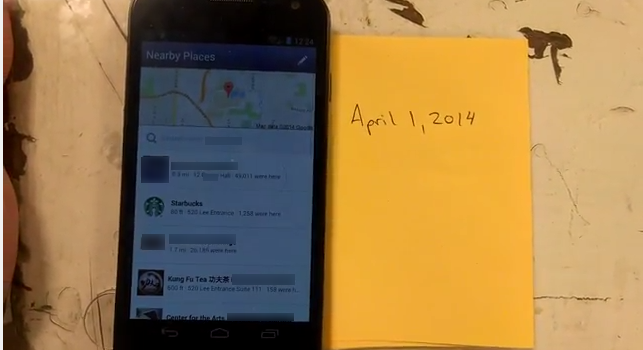
\includegraphics[width=2.33in]{./figures/apps/facebook/facebook3.png}
\caption{}
\end{subfigure}

\caption{\textbf{Mocking Facebook.} The screenshots show that we were able to
mock the Facebook app and initiate a check-in at Starbucks despite being a
half-mile away.}

\label{fig-mocking-facebook}

\end{figure*}

\begin{table}[t]
\begin{tabularx}{3.33in}{lX}
\textbf{App} & Facebook \\ \toprule
\textbf{Installs} & 500--1,000~million \\
\textbf{Mocking Objective} & Check-in at mocked location. \\
  \midrule
\textbf{Trace Length} & 1 minute 37 seconds \\
\textbf{Trace Size} & 268~K \\
\textbf{Location Mocks} & 106 \\
\textbf{Uses Sensors} & GPS, Accelerometer \\
\textbf{Sensor Mocks} & 2569 \\
\textbf{Wifi Scan Mocks} & 0 \\
\textbf{Cell Location Mocks} & 97 \\
\textbf{Video URL} & (Removed for blind review.) \\

\end{tabularx}

\caption{\textbf{Mocking Facebook.} Details of our Facebook mocking trace.}

\label{table-mocking-facebook}

\end{table}

\subsubsection{Mocking a game}

As a final mocking challenge, we attempted to use \PocketMocker{} to mock an
accelerometer-driven game. Fast Racing 3D is a car racing game available for
Android~\cite{fastracing-playstore-url}. Gaming is a popular activity on
smartphones, with studies showing that 32~\% of time spent on smartphones
being devoted to game play~\cite{flurry-smartphoneuse}. While \PocketMocker{}
normally records sensor data aggressively during recording in order to ensure
that it collects a superset of any information that could be requested during
the mocking session, games provide a particular challenge for replay due to
their aggressive use of high-rate sensor data---in this case, the
accelerometer.

Our objective in mocking Fast Racing was to use the mocked trace to control
gameplay during the mocking session. Users may want to mock apps for several
reasons: to avoid tedious replay of easier levels on apps that force players
to begin again after failing more difficult challenges, or to improve their
reputation through repetition when using apps that post scores to a public
leaderboard.

To mock Fast Racing gameplay we recorded a mocking trace of a portion of a
trip through one of the game's race courses.  This included tracking location,
connectivity, as well as sensor data from the accelerometer used to control
the vehicle. We then placed the smartphone on a desk, launched the Fast
Racing app, and initiated trace replay. Figure~\ref{fig-mocking-game} shows
three screenshots of Fast Racing being mocked demonstrating that the
accelerometer data was able to control the Fast Racing vehicle. For this
particular scenario, however, we found it difficult to trigger the mocking
replay at precisely the correct moment, with the associated time delay
causing the vehicle's path to eventually deviate from the original trace as
the mocking session continued. An anonymized video of our semi-successful
Fast Racing mocking session is also available at
\hyperlink{http://youtu.be/8fAj5dYFwS0}{\texttt{http://youtu.be/8fAj5dYFwS0}}.

\begin{figure*}[t]

\begin{subfigure}[t]{2.33in}
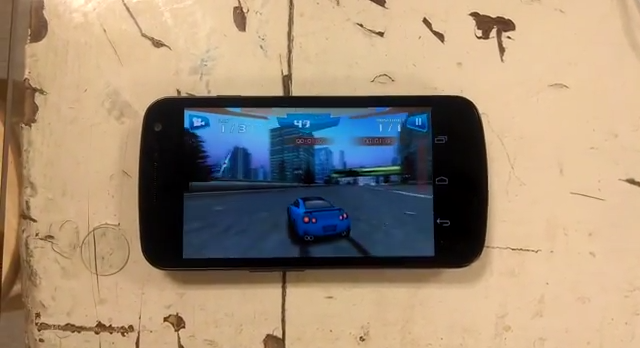
\includegraphics[width=2.33in]{./figures/apps/fast_racing/fastracing1.png}
\caption{}
\end{subfigure}%
\begin{subfigure}[t]{2.33in}
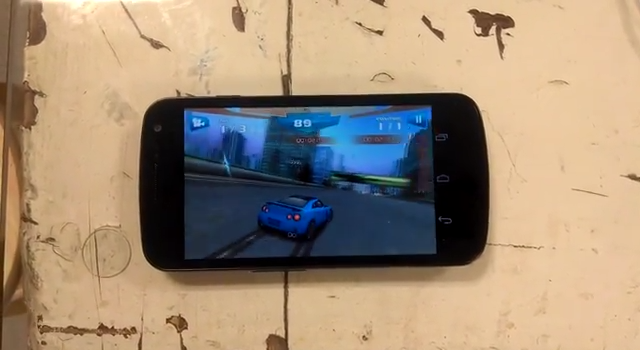
\includegraphics[width=2.33in]{./figures/apps/fast_racing/fastracing2.png}
\caption{}
\end{subfigure}%
\begin{subfigure}[t]{2.33in}
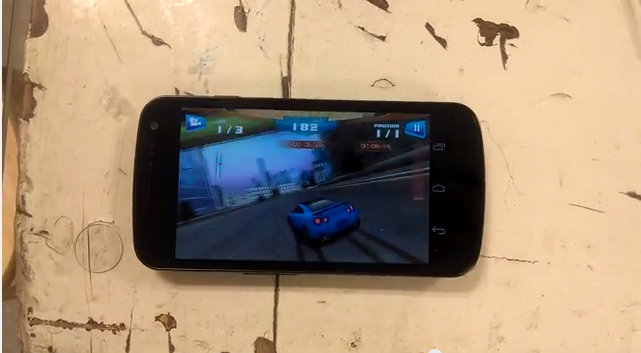
\includegraphics[width=2.33in]{./figures/apps/fast_racing/fastracing3.png}
\caption{}
\end{subfigure}

\caption{\textbf{Mocking Fast Racing.} The screenshots show that we were able
  to mock the accelerometer-driven Fast Racing game to control the vehicle
during the mocking session.}

\label{fig-mocking-game}

\end{figure*}

\begin{table}[t]

\begin{tabularx}{3.33in}{lX}
\textbf{App} & Fast Racing 3D \\ \toprule
\textbf{Installs} & 50--100~million \\
  \textbf{Mocking Objective} & Control game play \\ \midrule
\textbf{Uses Sensors} & Accelerometer \\
\textbf{Trace Length} & 1 minute 35 seconds \\
\textbf{Trace Size} & 296~K \\
\textbf{Location Mocks} & 96 \\
\textbf{Uses Sensors} & GPS, Accelerometer \\
\textbf{Sensor Mocks} & 1363 \\
\textbf{Wifi Scan Mocks} & 96 \\
\textbf{Cell Location Mocks} & 96 \\
\textbf{Video URL} &
  \hyperlink{http://youtu.be/8fAj5dYFwS0}{\texttt{http://youtu.be/8fAj5dYFwS0}}
  \\

\end{tabularx}

\caption{\textbf{Mocking Fast Racing.} Details of our Fast Racing
  mocking trace.}

\label{table-mocking-game}
\vspace*{-0.2in}
\end{table}


\subsubsection{Mocking overhead}
\label{subsec-overhead}

\begin{figure*}[t]

\begin{subfigure}[t]{2.33in}
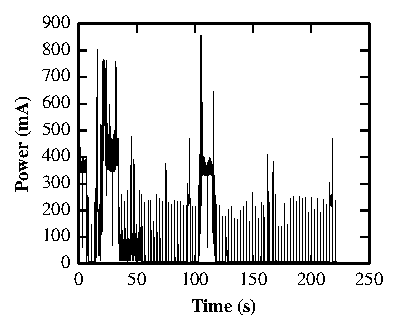
\includegraphics[width=2.33in]{./figures/overhead/idle.pdf}
\caption{Idle power consumption.}
\label{fig-overhead-idle}
\end{subfigure}%
\begin{subfigure}[t]{2.33in}
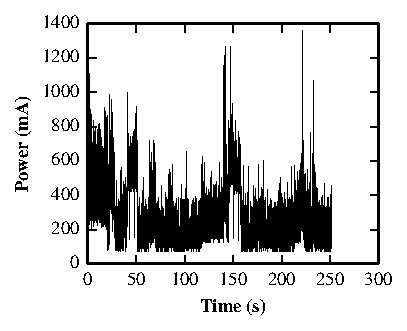
\includegraphics[width=2.33in]{./figures/overhead/recording.pdf}
\caption{Recording power consumption.}
\label{fig-overhead-recording}
\end{subfigure}%
\begin{subfigure}[t]{2.33in}
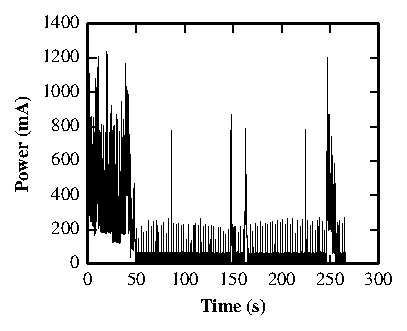
\includegraphics[width=2.33in]{./figures/overhead/replaying.pdf}
\caption{Replaying power consumption.}
\label{fig-overhead-replaying}
\end{subfigure}

\caption{\textbf{\PocketMocker{} Overhead.} Power usage is high during the
record phase while \PocketMocker{} rapidly gathers all data that might be
needed during the mocking session. Replay (\ref{fig-overhead-replaying})
power usage is typical of normal smartphone operation, with the screen going
off after 40~s.}

\label{fig-overhead}

\end{figure*}

% 03 Apr 2014 : GWA : ND TODO : Sanity check this... I'm writing without a
% figure :-).

To address an inevitable concern about the mocking process, we measured the
energy usage of \PocketMocker{} while recording and replaying context traces.
We measured the energy consumption of \PocketMocker{} using the Monsoon Power
Monitor~\cite{monsoon-url} attached to our Galaxy Nexus smartphone. Because
\PocketMocker{} records certain types of data only when triggered by a
location update, we mounted the entire setup on a cart so that the phone
could be moved during the measurement of the trace collection process.

Figure~\ref{fig-overhead} shows the power measured by the Monsoon. The first
trace segment is a baseline showing idle power consumption. The second trace
shows power consumption during the recording process, and the third shows
replay. Because \PocketMocker{} rapidly samples data from all available
sensors during the trace recording process, this naturally leads to high
energy usage, as shown in Figure~\ref{fig-overhead-recording}. During replay,
however, mocking produces little overhead and energy usage is typical, as
shown in Figure~\ref{fig-overhead-replaying}. Because users must only record
a trace one time but then can replay it multiple times, we consider the high
overhead of trace recording to be acceptable. We are also designing further
optimizations to reduce energy usage while replaying context traces, as
because mocked data is being used real sensors---including power-hungry ones
such as the GPS---can be disabled.

Mocking traces also consume disk space to store, with our experiments
indicating that \PocketMocker{}'s traces consume roughly 3~K per second
without removing repeated readings or performing compression. This means that
1~GB of disk space would allow a user to record almost 100~hours of mocking
traces.

\subsection{Users Can Use \PocketMocker{}}
\label{subsec-usability}

% 03 Apr 2014 : GWA : ND TODO : 1 column (0.5 page) about the experiment.
% Describe the app, what it does, how many people participated, etc. Then
% some bits of the qualitative feedback.

With positive results from our previous survey and a prototype implemented, we 
wanted to gain a qualitative insight to future users of \PocketMocker{}. Over 
the course of one day, we had 7 users use our most recent record-and-replay 
prototype. Due to physical limitations, we studied users individually with one 
Galaxy Nexus smartphone. 

After receiving some background information on the project and instructions
on how to use \PocketMocker{}, users were given the smartphone with the goal
of tricking an open-source Pedometer~\cite{pedometer-playstore-url} that they
were walking (and being active beings), while the phone was sitting on the
desk in the lab. We wanted to receive feedback on the app, the idea,
and the process, so we collected responses to the following questions after
they saw \PocketMocker{} in action: ``Did DataDecoy mock the Pedometer?'' and
``Comments?''. All users reacted positively, with one who ``would love to use
it for some other apps'' and 42\% of our users believe it has strong
``potential''. One user was so elated that he exclaimed ``Much awesome, very
app!''.

The users found the app and process to be extremely transparent: all
that was needed was to open the app, create an objective, hit record, and
forget about it. In all cases, \PocketMocker{} was able to trick the
Pedometer into classifying the phone's action as walking---by showing steps
increase---when the phone was really sitting idle on a desk.

\begin{table}[t]

\begin{framed}
  \textbf{What can data collected by your smartphone reveal about you?}

  {\small The questions below assess how much you think your phone is able to
    determine about you without asking. All the questions assume that you
    have installed the application and granted it the permissions it
  requested.}
  \vspace*{-5pt}

  \begin{itemize}[leftmargin=15pt,noitemsep]
    \item \uline{Without asking, what could an application determine about} your
      yearly income?
      \begin{itemize}[leftmargin=15pt,noitemsep]
        \item An application could predict my income exactly, to within \$1 /
          year.
        \item An application could predict my income to within \$100 / year.
        \item An application could predict my income to within \$10,000 / year.
        \item An application could not determine anything about my income
          level.
      \end{itemize}
    \item $\ldots$ your weight?
    \item $\ldots$ your social network?
    \item $\ldots$ your activity level?
    \item $\ldots$ where you live?
  \end{itemize}

  \vspace*{-10pt}

\end{framed}

\begin{framed}
  \textbf{What are you comfortable with applications knowing about you?}

  {\small The questions below assess how comfortable you are with smartphone
    application being able to determine the same things about you we asked
    about in the first section. \textbf{Please indicate your comfort level
  between not comfortable at all (1) and completely comfortable (5).}}
  \vspace*{-5pt}

  \begin{itemize}[leftmargin=15pt,noitemsep]
    \item \uline{How comfortable are you with smartphone applications
      knowing} your yearly income?
    \item $\ldots$ your weight?
    \item $\ldots$ about your social network?
    \item $\ldots$ your activity level?
    \item $\ldots$ where you live?
  \end{itemize}
  \vspace*{-10pt}

\end{framed}

\begin{framed}
  \textbf{Would you like to alter what your smartphone knows about you?}

  {\small These questions assess your interest in altering what your
    smartphone knows about you. Assume that a system exists that would allow
  you to change the qualities as indicated by the questions.}
  \vspace*{-5pt}

  \begin{itemize}[leftmargin=15pt,noitemsep]
    \item \uline{If a smartphone application could accurately determine} my income
      level 
      \begin{itemize}[leftmargin=15pt,noitemsep]
        \item I would like to appear to have a lower yearly income than I
          actually do.
        \item I would like to appear to have a higher yearly income than I
          actually do.
        \item I am comfortable revealing my true income level to the
          application.
      \end{itemize}
    \item $\ldots$ my weight
    \item $\ldots$ my social network
    \item $\ldots$ my activity level
    \item $\ldots$ where I live
  \end{itemize}
  \vspace*{-10pt}

\end{framed}


\caption{\textbf{Mocking survey questions.} Respondents were asked three
groups of questions about five aspects of their personal lives their
smartphone could observe. For each group one sample question and answers is
shown.}

  \label{table-surveyquestions}
\end{table}
